Figure \ref{fig:img1_src} shows the first image which has to be restored. This image is compared to the original  (Figure \ref{fig:orignal}) much darker.  Based on the histogram  it can be seen that a large amount of black pixels appear to be on the image.  The image affected by pepper noise.  

\begin{figure}[H]
    \centering
    \begin{subfigure}[b]{0.23\textwidth}
        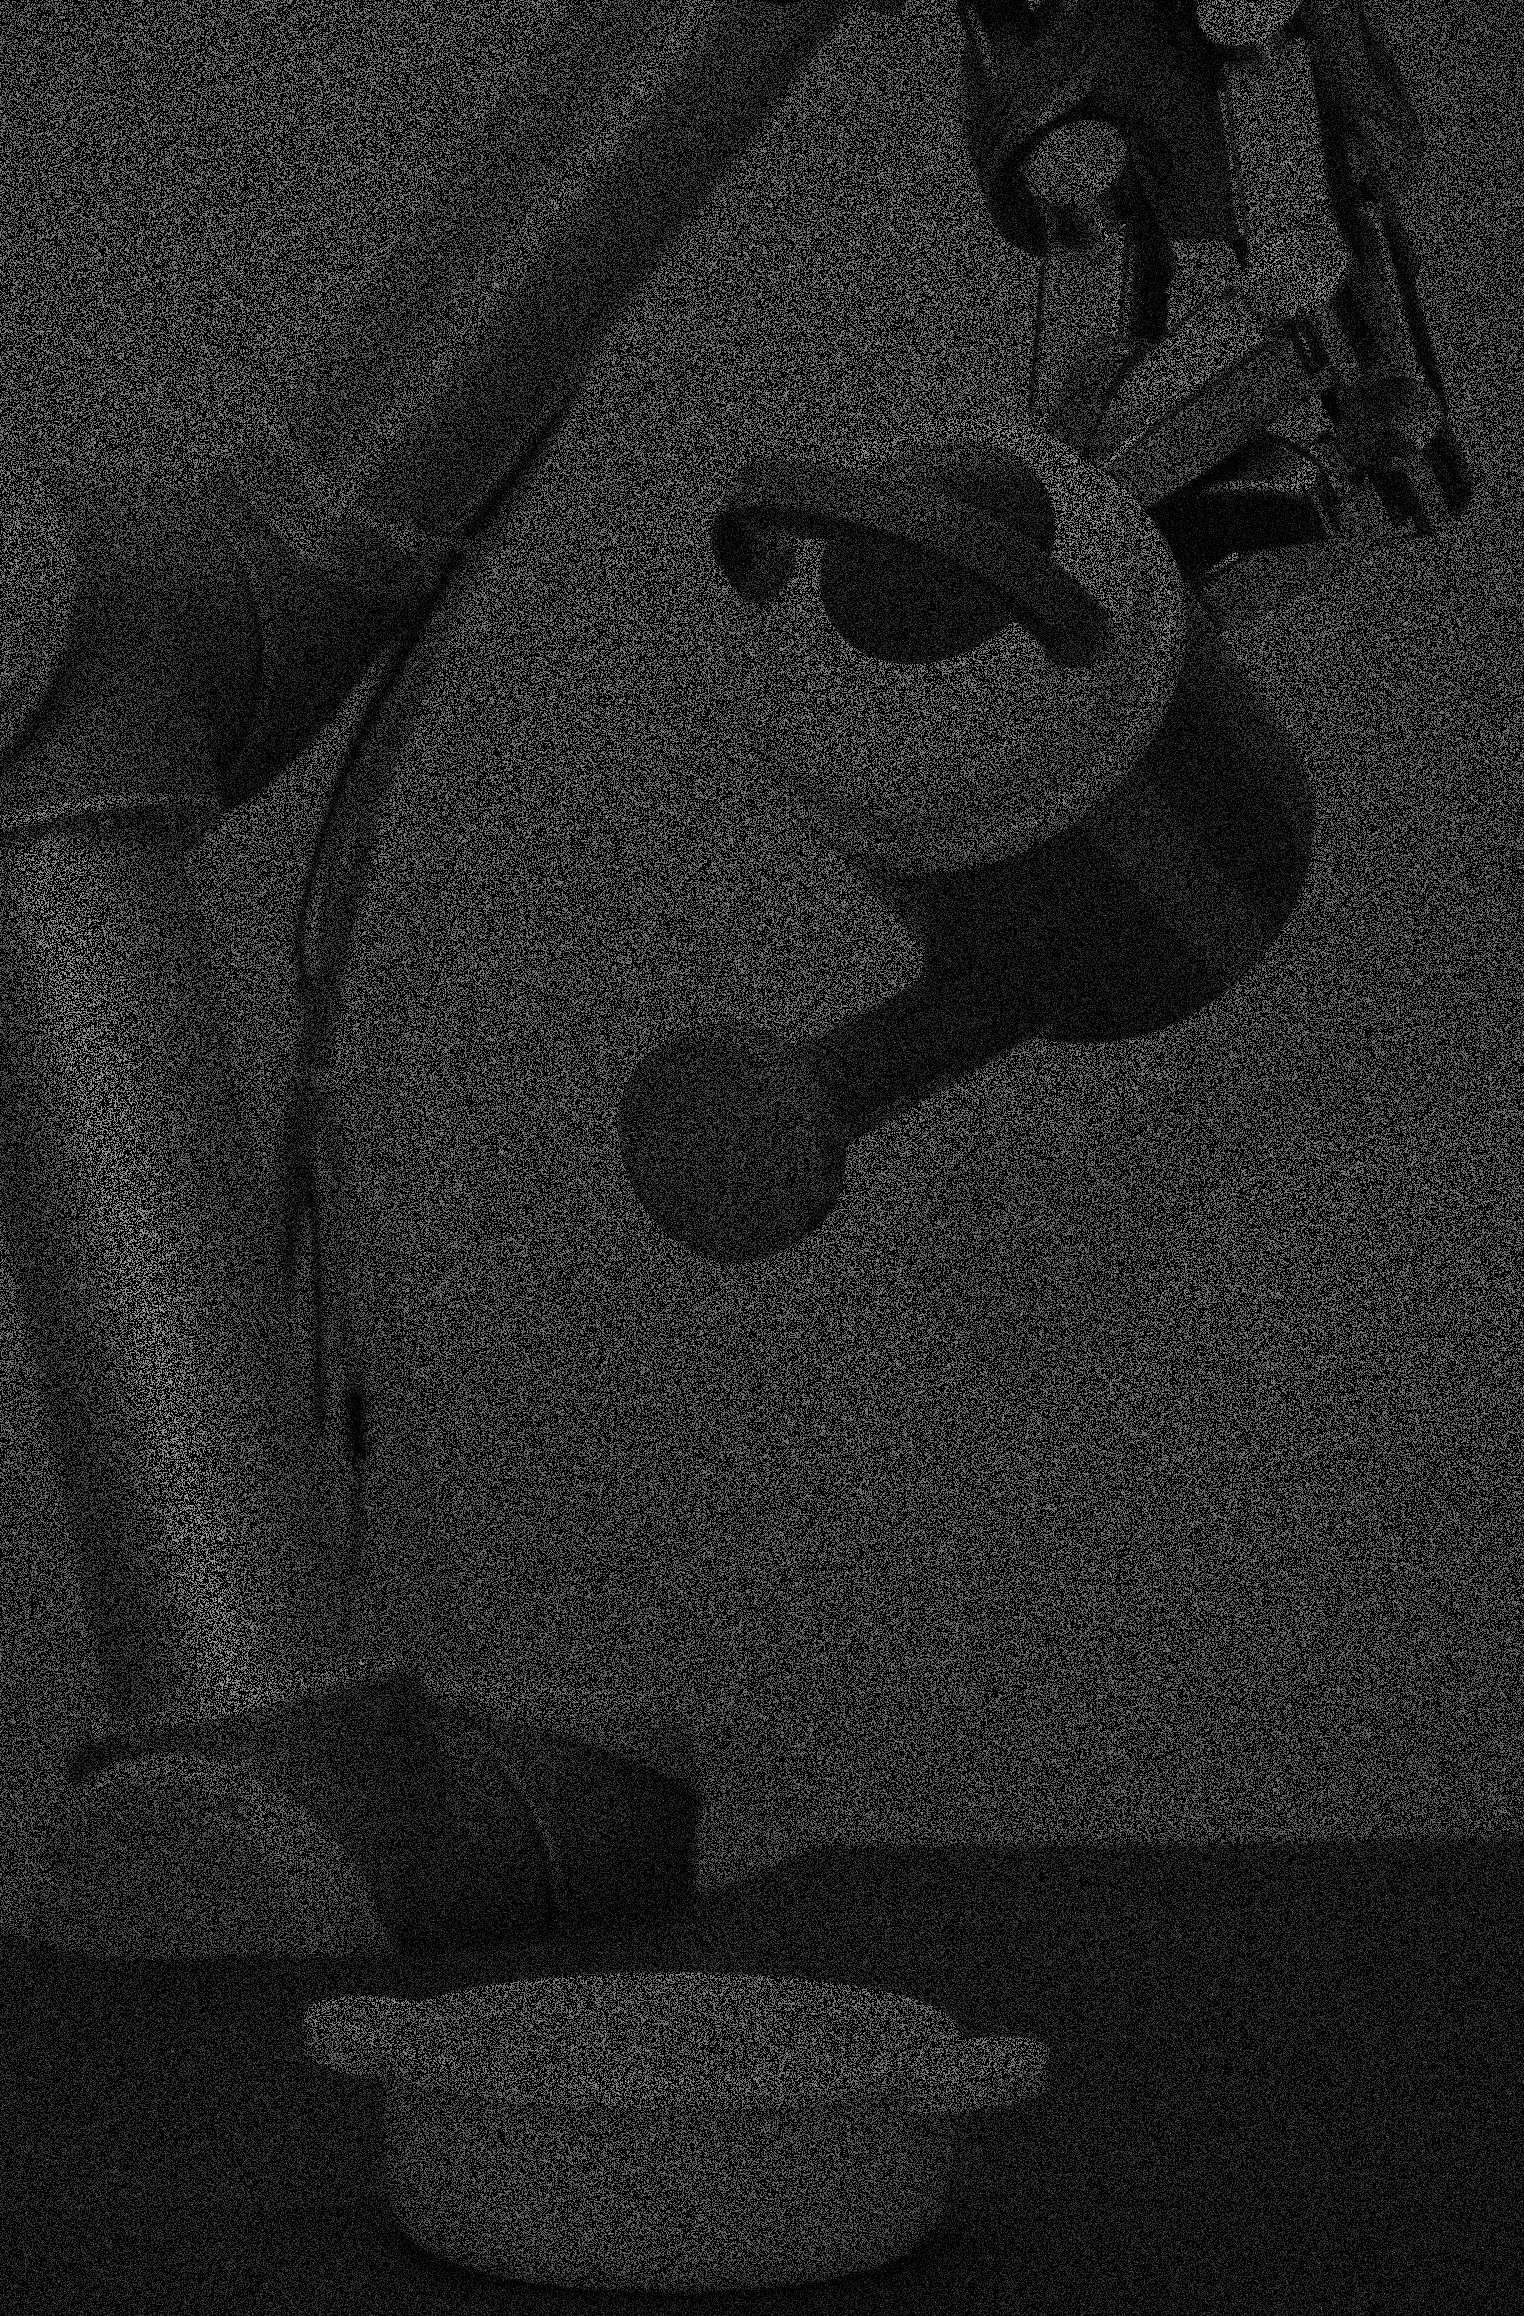
\includegraphics[width=\textwidth]{img1/Image1.png}
        \caption{Image1 with \\no restoration}
        \label{fig:img1_src}
    \end{subfigure}
    \begin{subfigure}[b]{0.446\textwidth}
        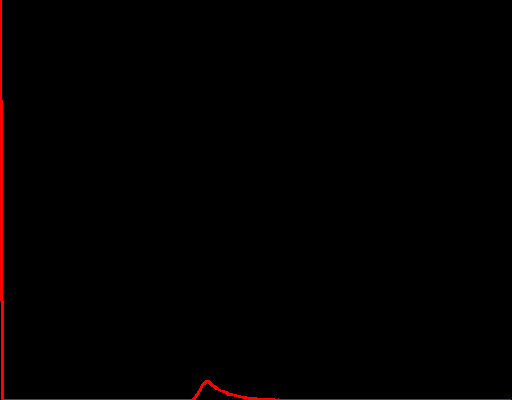
\includegraphics[width=\textwidth]{img1/src_hist.png}
        \caption{Histogram of Image1}
        \label{fig:img1_hist}
    \end{subfigure}
    \caption{Analysis of image 1}\label{fig:img1}
\end{figure}

An effective way of removing salt and pepper noise it to use an median filter, which would take the median value  of fixed numbered  values and assign it to that pixel position, but as the amount of pepper noise is too large, would an median value mostly lead to a black pixel, hence not provide that much of an improvement as seen in Figure \ref{fig:img_median_full}.  

\begin{figure}[H]
    \centering
    \begin{subfigure}[b]{0.27\textwidth}
        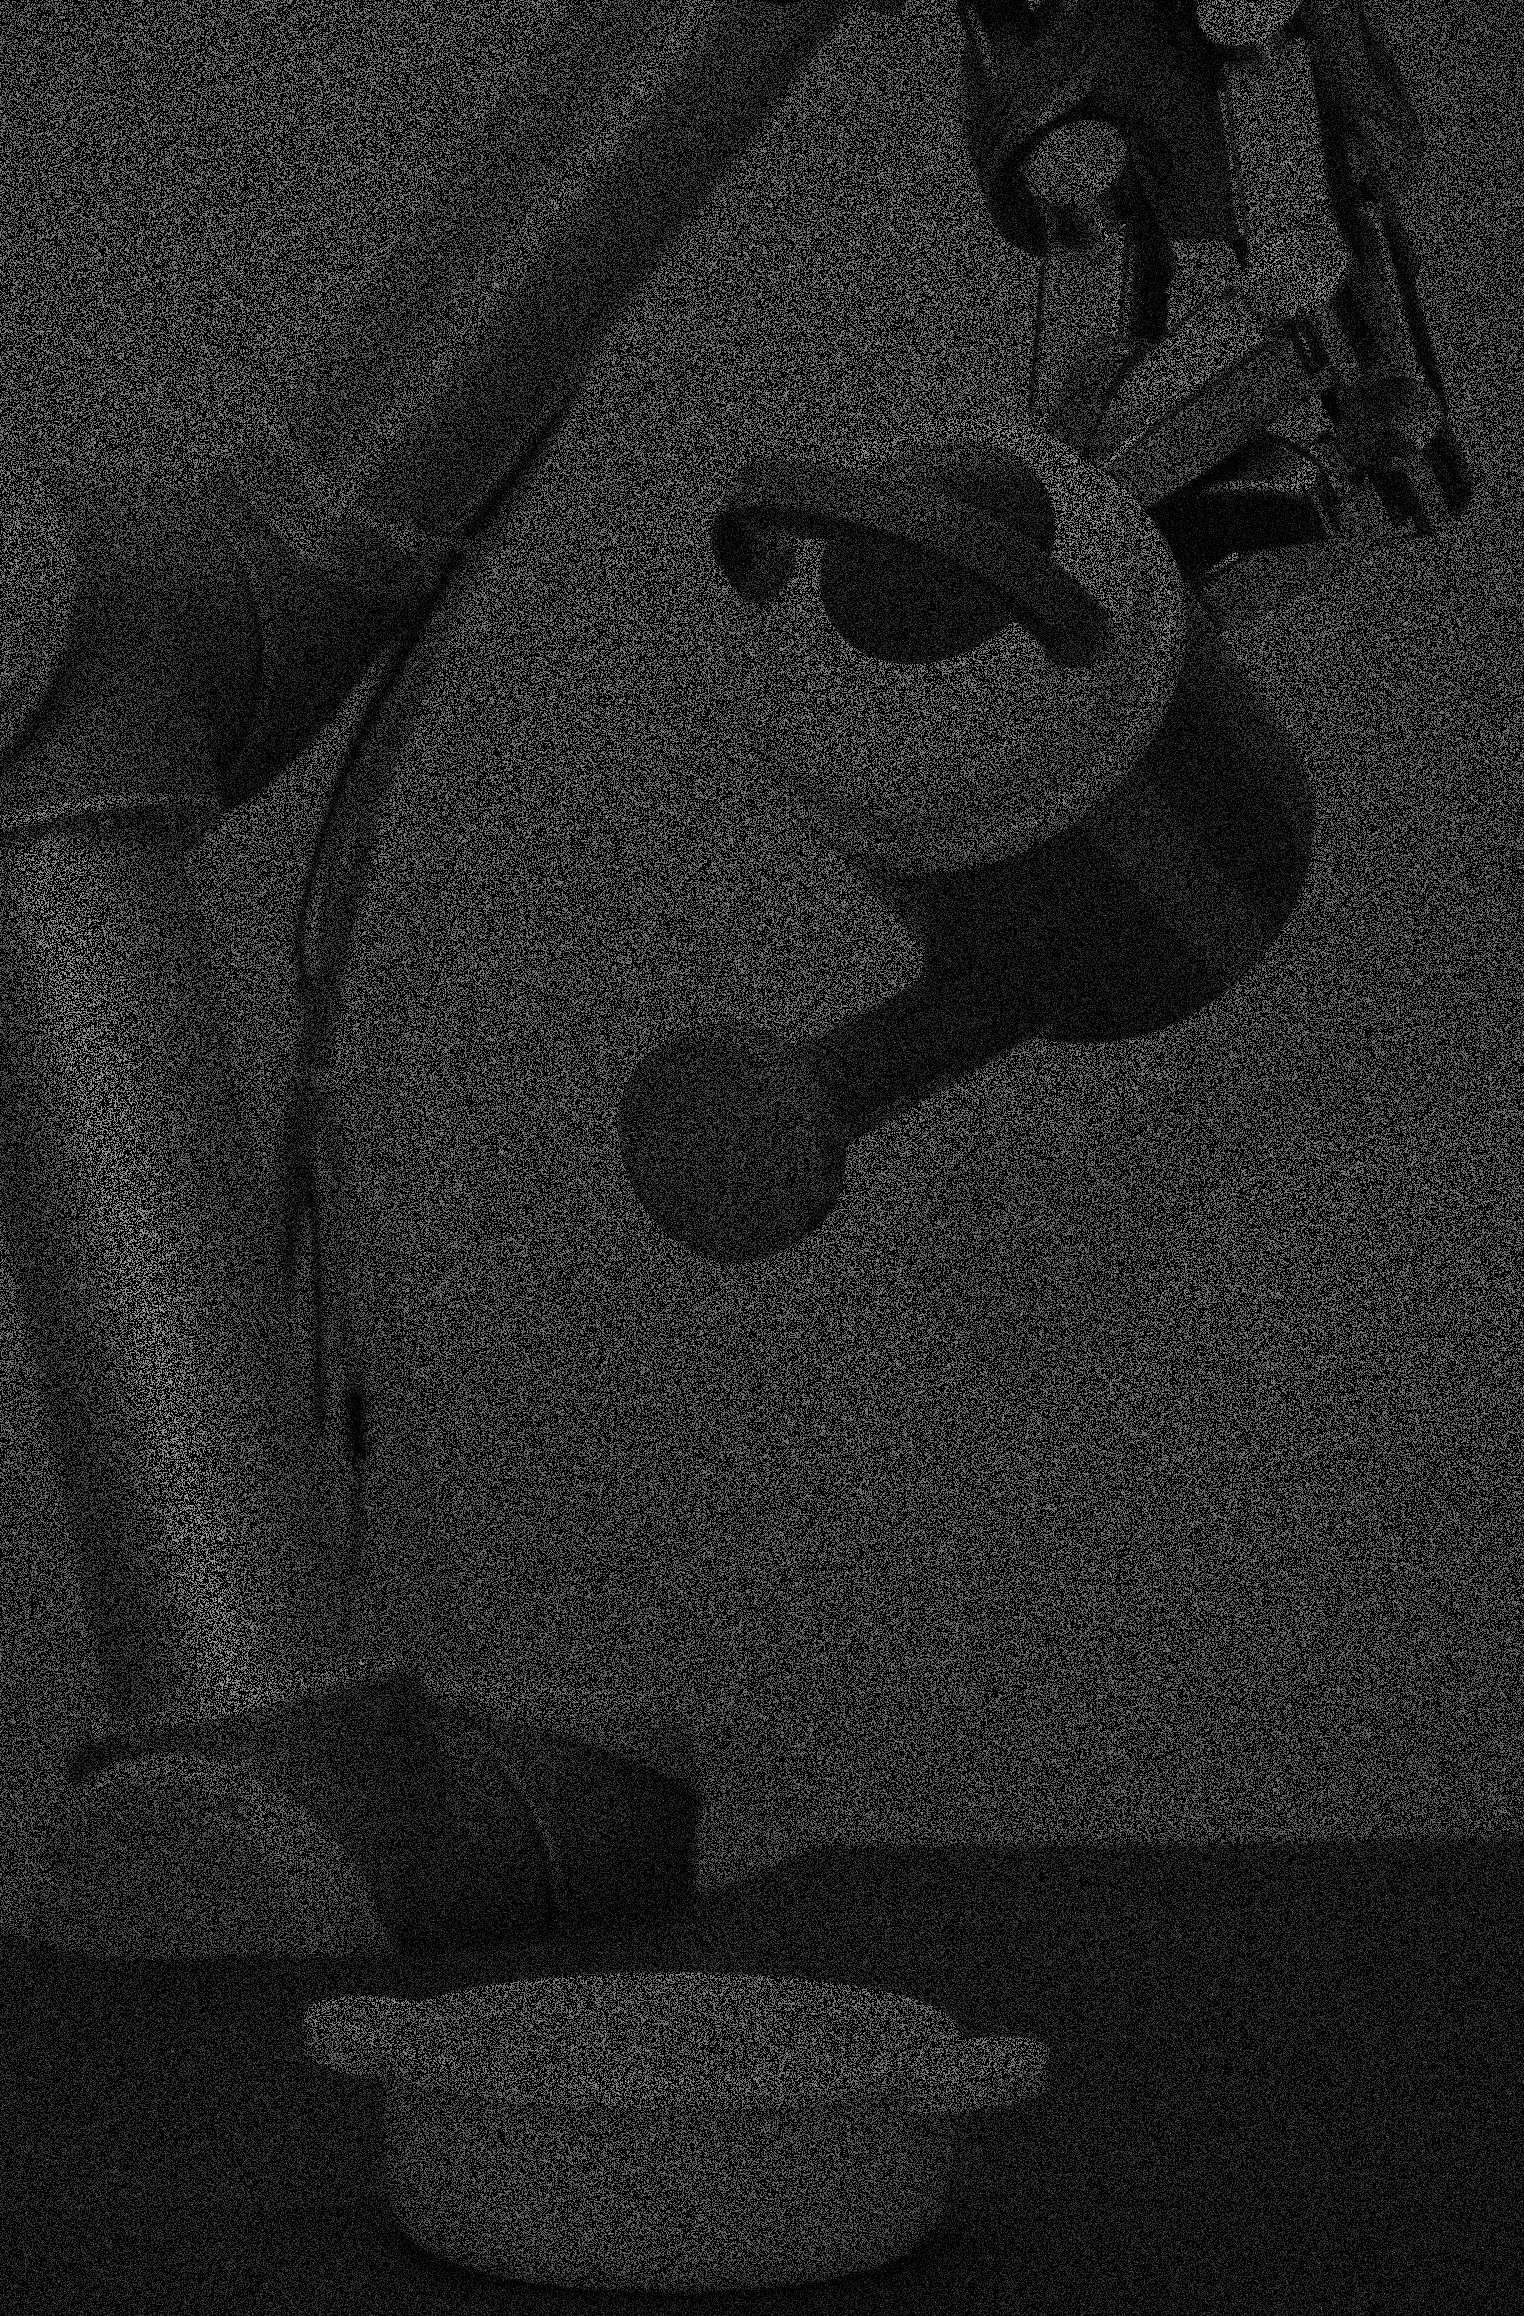
\includegraphics[width=\textwidth]{img1/Image1.png}
        \caption{Image1 with \\no restoration}
        \label{fig:img1_src}
    \end{subfigure}
    \begin{subfigure}[b]{0.27\textwidth}
        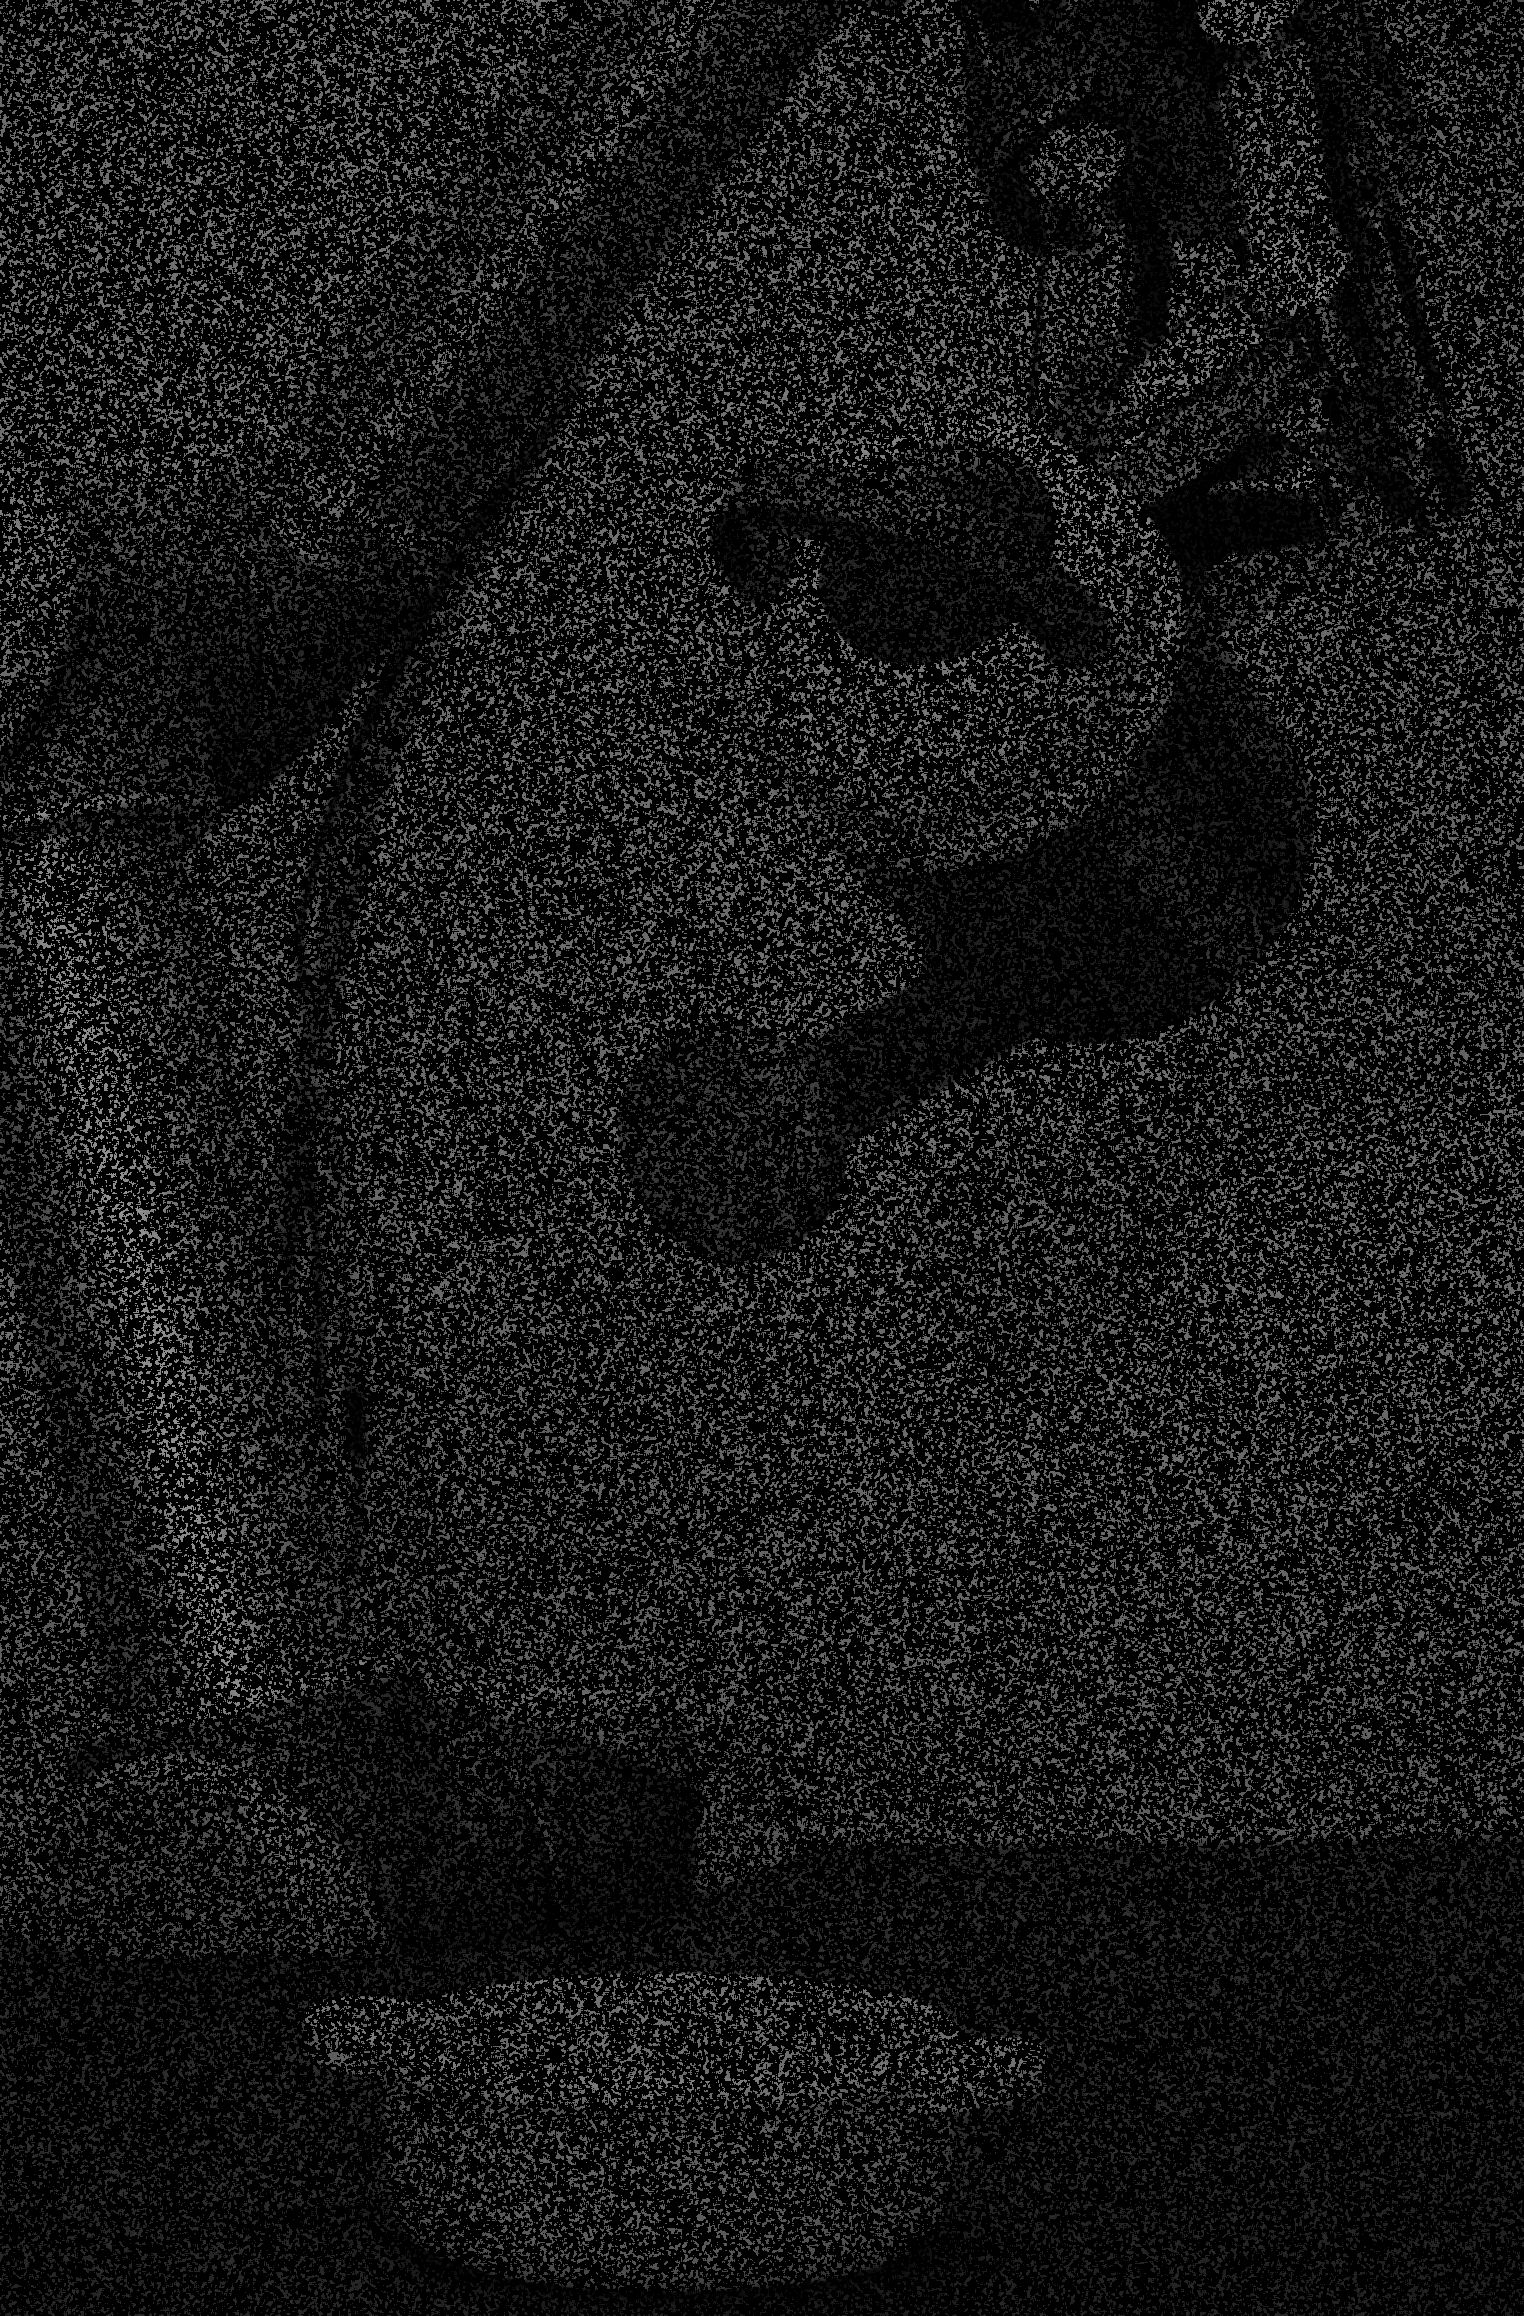
\includegraphics[width=\textwidth]{img1/img_1_medianBlur_3.png}
        \caption{Image1 filtered with median filter kernelsize 3}
        \label{fig:img1_median3}
    \end{subfigure}
       \begin{subfigure}[b]{0.27\textwidth}
        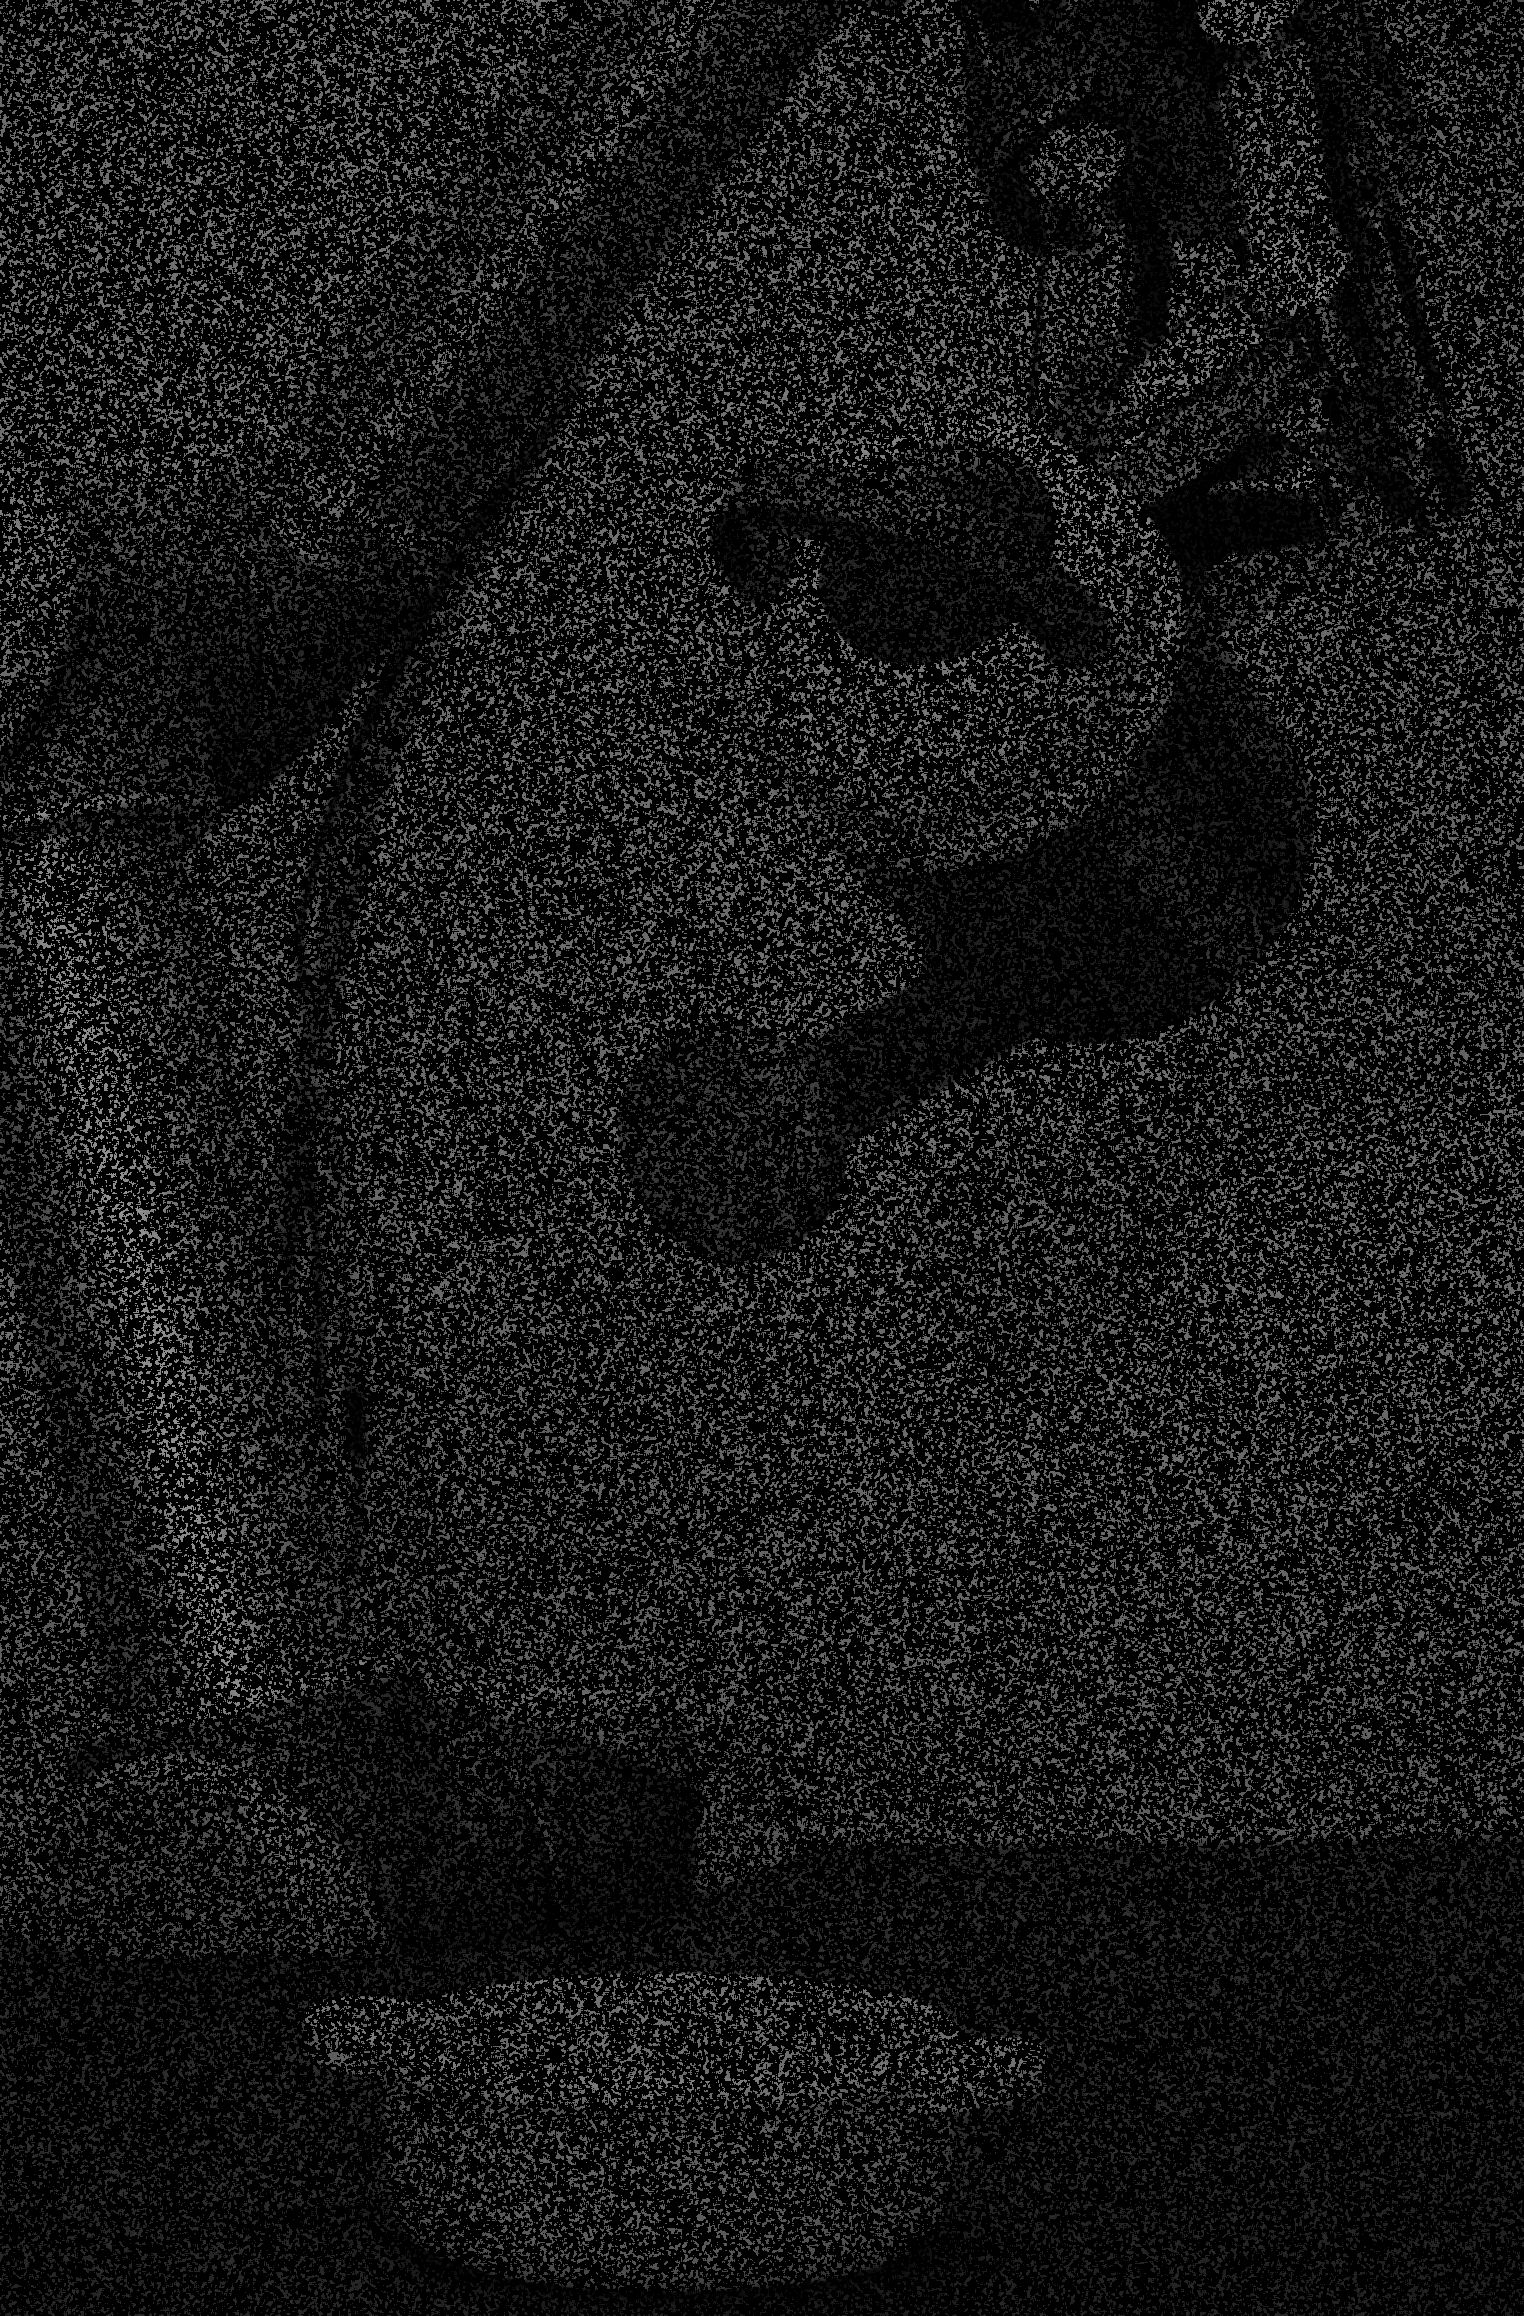
\includegraphics[width=\textwidth]{img1/img_1_medianBlur_9.png}
        \caption{Image1 filtered with median filter kernelsize 9}
        \label{fig:img1_median9}
    \end{subfigure}
    \caption{Median filter applied to image1}\label{fig:img_median_full}
\end{figure}


\end{document}